\documentclass[usenames,dvipsnames,aspectratio=169]{beamer}

\usepackage[utf8]{inputenc}
\usepackage[T1]{fontenc}
\usepackage[magyar]{babel}
\usepackage{indentfirst}
\usepackage{listingsutf8}
\lstset{literate=
  {á}{{\'a}}1 {é}{{\'e}}1 {í}{{\'i}}1 {ó}{{\'o}}1 {ú}{{\'u}}1
  {Á}{{\'A}}1 {É}{{\'E}}1 {Í}{{\'I}}1 {Ó}{{\'O}}1 {Ú}{{\'U}}1
  {à}{{\`a}}1 {è}{{\`e}}1 {ì}{{\`i}}1 {ò}{{\`o}}1 {ù}{{\`u}}1
  {À}{{\`A}}1 {È}{{\'E}}1 {Ì}{{\`I}}1 {Ò}{{\`O}}1 {Ù}{{\`U}}1
  {ä}{{\"a}}1 {ë}{{\"e}}1 {ï}{{\"i}}1 {ö}{{\"o}}1 {ü}{{\"u}}1
  {Ä}{{\"A}}1 {Ë}{{\"E}}1 {Ï}{{\"I}}1 {Ö}{{\"O}}1 {Ü}{{\"U}}1
  {â}{{\^a}}1 {ê}{{\^e}}1 {î}{{\^i}}1 {ô}{{\^o}}1 {û}{{\^u}}1
  {Â}{{\^A}}1 {Ê}{{\^E}}1 {Î}{{\^I}}1 {Ô}{{\^O}}1 {Û}{{\^U}}1
  {œ}{{\oe}}1 {Œ}{{\OE}}1 {æ}{{\ae}}1 {Æ}{{\AE}}1 {ß}{{\ss}}1
  {ç}{{\c c}}1 {Ç}{{\c C}}1 {ø}{{\o}}1 {å}{{\r a}}1 {Å}{{\r A}}1
  {€}{{\EUR}}1 {£}{{\pounds}}1 {ő}{{\H{o}}}1 {ű}{{\H{u}}}1
}
\lstdefinestyle{HTML}{
  language=HTML,
  breaklines=true,
  postbreak=\mbox{\textcolor{red}{$\hookrightarrow$}\space},
  stringstyle=\ttfamily,
  inputencoding=utf8
}
\usepackage{hyperref}
\usepackage{attachfile}
\usepackage{multirow}
% Navigációs pöttyök hozzáadása subsection nélküli fejezetekhez
\usepackage{remreset}
\makeatletter
\@removefromreset{subsection}{section}
\makeatother
\setcounter{subsection}{1}
%%%%%
\attachfilesetup{color={1.0 0.6 0.0},author={HFM},description={Kattintson duplán a minta %
megtekintéséhez!},icon=Paperclip}
\definecolor{kiemelesszin}{rgb}{0.6,0.0,0.0}
\definecolor{kiemelesszinZ}{rgb}{0.0,0.6,0.0}
\definecolor{kiemelesszinN}{RGB}{196,127,0}
\definecolor{hivatkozasszin}{rgb}{0.0,0.0,0.75}
\newcommand{\kiemel}[1]{{\color{kiemelesszin}#1}}
\newcommand{\kiemelZ}[1]{{\color{kiemelesszinZ}#1}}
\newcommand{\kiemelN}[1]{{\color{kiemelesszinN}#1}}
\newcommand{\hiv}[1]{{\color{hivatkozasszin}#1}}
\frenchspacing
\usetheme[compress]{Berlin}

\title[Web technológiák - HTML]{Egyszerű HTML5 weboldalak készítése}
\subtitle{(GKxB\_INTM049)}
\author{Dr. Hatwágner F. Miklós}
\institute{Széchenyi István Egyetem, Győr}
\date{\hiv{\href{https://github.com/wajzy/GKxB\_INTM049.git}{https://github.com/wajzy/GKxB\_INTM049.git}}\\ \today}

\begin{document}

%1
\begin{frame}[plain]
  \titlepage
\end{frame}

\section{Jelölőnyelvek}

%2
\begin{frame}
  \begin{itemize}
    \item Cél: a nyers szöveg egyes részeit strukturálni, jelentésbeli többletet hozzáadni (pl. fejezetcím, bekezdés)
    \item Történeti előzmény: nyomdai előkészítés, kéziratok szerkesztése, gépi szedőrendszerek
    \item Példák jelölőnyelvekre: 
      \hiv{\href{http://man7.org/linux/man-pages/man7/roff.7.html}{roff}}, 
      \hiv{\href{https://www.latex-project.org/}{LaTeX}}, 
      \hiv{\href{https://en.wikipedia.org/wiki/Standard_Generalized_Markup_Language}{SGML}}
  \end{itemize}
\end{frame}

\subsection{roff}

%3
\begin{frame}
  \footnotesize
  \begin{description}[m]
    \item[RUNOFF] \hfill \\ nyers szövegből és parancsokból (.XX) álló fájlok $\to$ tördelt megjelenítés buta terminálokon (OS: Compatible Time Sharing System, CTSS, 1963)
    \item[runoff] \hfill \\ a RUNOFF bővített képességű portja \emph{IBM Selectric} terminálokhoz (OS: Multiplexed Information and Computing Service, multics, $\approx$'60-as évek vége)
    \item[roff] \hfill \\ a runoff továbbfejlesztése a Bell Telephone Labs-nál (1973) a PDP-11 géphez kapcsolt \emph{Graphic Systems CAT} (grafikus szedőegység) miatt. A roff család:
    \begin{description}[m]
      \item[troff] \hfill \\ typesetter roff a CAT-hez
      \item[nroff] \hfill \\ terminálokhoz és nyomtatókhoz
      \item[roff] \hfill \\ korlátozott képességű runoff utód, nem fejlesztették tovább
    \end{description}
    \item[groff] \hfill \\ GNU implementáció, máig fejlesztik $\to$ man oldalak
  \end{description}
\end{frame}

%4
\begin{frame}
  \begin{columns}[c]
    \column{0.5\textwidth}
      \tiny
      \begin{exampleblock}{\textattachfile{groff.1}{/usr/share/man/man1/groff.1.gz/groff.1}}
        \lstinputlisting[language=,breaklines=true,linerange={1-3},numbers=left,firstnumber=1]{groff.1}
        \lstinputlisting[language=,basicstyle=\ttfamily,breaklines=true,postbreak=\mbox{\textcolor{red}{$\hookrightarrow$}\space},linerange={75-85},numbers=left,firstnumber=75]{groff.1}
      \end{exampleblock}
    \column{0.5\textwidth}
      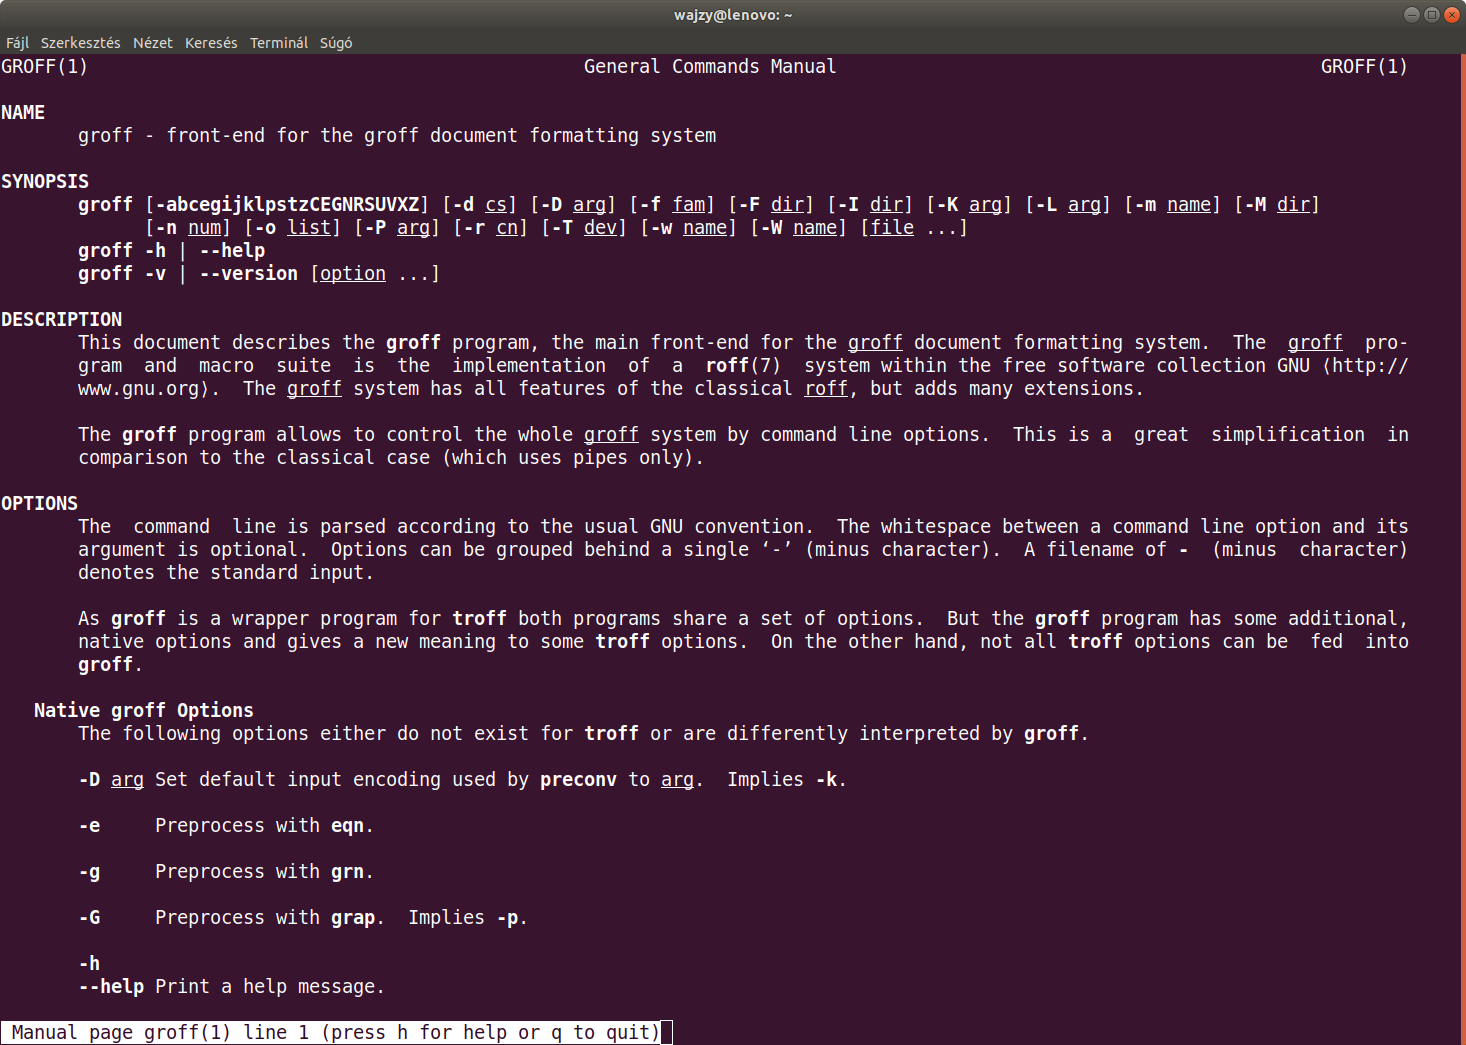
\includegraphics[width=\linewidth]{./groff.png}
  \end{columns}
\end{frame}

\subsection{\LaTeX{}}

%5
\begin{frame}
  \begin{columns}[T]
    \column{0.3\textwidth}
      \begin{description}[m]
        \item[\TeX] \hfill \\ Betűszedő rendszer, fejlesztője Donald E. Knuth, 1978 (Elégedetlenség \hiv{\href{https://www-cs-faculty.stanford.edu/~knuth/taocp.html}{könyvének}} szedésével.)
        \item[\LaTeX] \hfill \\ \TeX-en alapuló szövegformázó rendszer, Leslie Lamport, 1983
      \end{description}
    \column{0.7\textwidth}
        \begin{exampleblock}{\textattachfile{html.tex}{html.tex}}
          \centering
          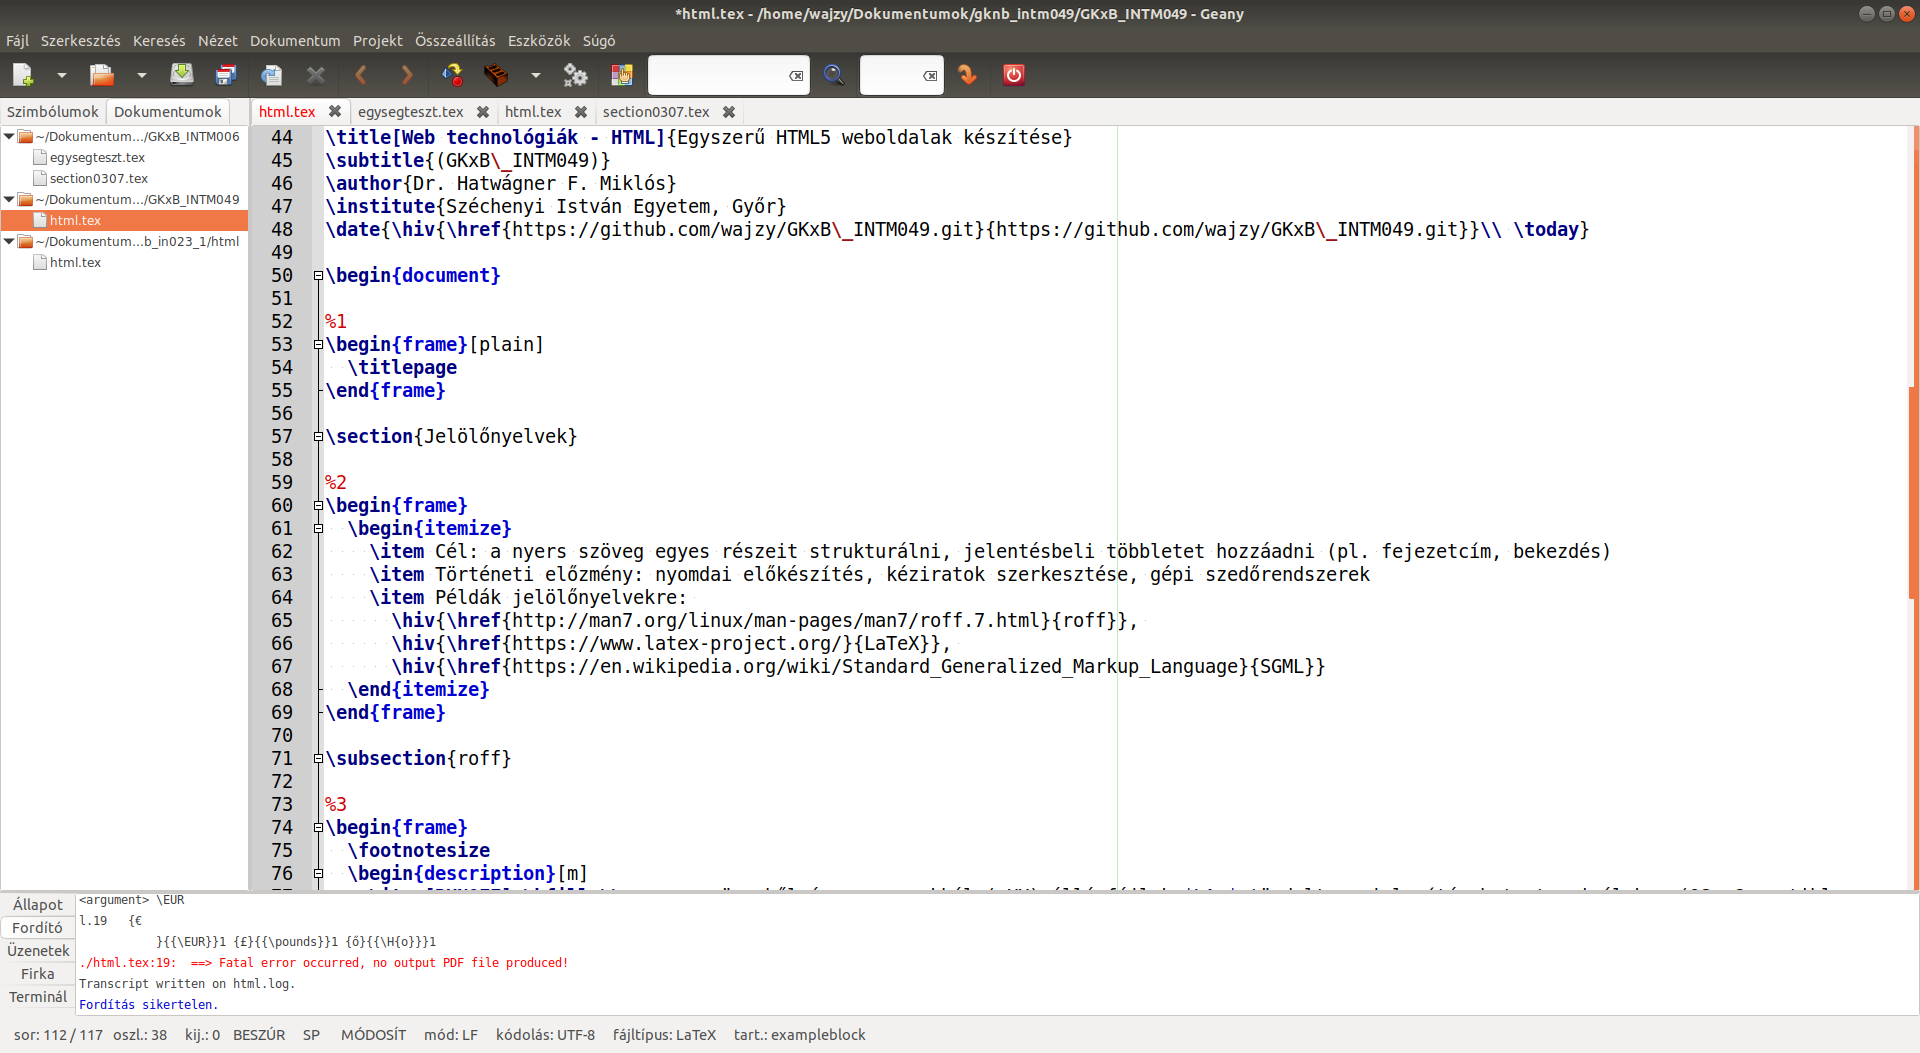
\includegraphics[scale=.14]{./latex.png}
        \end{exampleblock}
  \end{columns}
\end{frame}

\subsection{SGML}

%6
\begin{frame}
  \begin{itemize}
    \item SGML (Standard Generalized Markup Language), ISO 8879:1986
    \item Szabványos jelölőnyelv dokumentumok szerkezetének leírására,
beleértve a címkék definiálását is
    \item Gépfüggetlen metanyelv
    \item Előzménye: GML (1969)
    \begin{itemize}
      \item C. \kiemel{G}oldfarb (IBM), E. \kiemel{M}osher, R. \kiemel{L}orie
      \item dokumentumtípusonként egyedi kódolási séma definiálható
      \item előre definiált elemek egymásba ágyazhatóak
      \item először az IBM nyomdarendszere használta
    \end{itemize}
    \item Tulajdonságai
    \begin{itemize}
      \item Deklaratív: struktúrát és attribútumokat rögzít, nem a feldolgozás módját ($\to$~időtállóság)
      \item Gépi feldolgozás lehetősége
    \end{itemize}
  \end{itemize}
\end{frame}

%7
\begin{frame}
  \begin{itemize}
    \item Legfontosabb építőelemek
    \begin{itemize}
      \item Elemek ([element] nyitó és záró cimkék [tag] által határolva)
      \item A nyitó tagben attribútumok (kulcs-érték párok) adhatók meg
      \item Elemek egymásba ágyazhatóak
      \item Elemek, attribútumok alkalmazási szabályai $\to$ Document Type Definition (DTD)
    \end{itemize}
    \item Néhány korai, jelentős alkalmazás
    \begin{itemize}
      \item Electronic Manuscript Project of the Association of American Publishers (AAP, tudományos dokumentumok)
      \item Computer-aided Acquisition and Logistic Support (CALS, katonai dokumentumok kezelése)
      \item LinuxDoc (Linux csomagok)
    \end{itemize}
  \end{itemize}
\end{frame}

%8
\begin{frame}[fragile]
  \scriptsize
  \begin{columns}[T]
    \column{0.4\textwidth}
    \begin{exampleblock}{SGML példa}
      \begin{verbatim}
<!DOCTYPE PEOPLE SYSTEM 
  "people.dtd">
<PEOPLE DATE="15 6 2000">
 <NAME TITLE="Mr">
  <FIRST>Wally</FIRST>
  <LAST>Wallpaper</LAST>
 </NAME>
 <NAME>
  <LAST>Jackson</LAST>
 </NAME>
 <NAME TITLE="Dr">
  <FIRST>Susan</FIRST>
  <MIDDLE>Ramsay</MIDDLE>
  <LAST>Sukie</LAST>
 </NAME>
</PEOPLE>
\end{verbatim}
    \end{exampleblock}
    \column{0.6\textwidth}
    \begin{exampleblock}{people.dtd}
      \begin{verbatim}
<!ELEMENT people - - (name+)>
<!ATTLIST people date NUMBERS #REQUIRED>

<!ELEMENT name - - (first?, middle?, last)>
<!ATTLIST name title CDATA #IMPLIED>

<!ELEMENT first - - (#PCDATA)>
<!ELEMENT middle - - (#PCDATA)>
<!ELEMENT last - - (#PCDATA)>
\end{verbatim}
    \end{exampleblock}
    \tiny
    Forrás: \textattachfile{chap4.html}{OmniMark dokumentáció}
  \end{columns}
\end{frame}

\subsection{A HTML története}

%9
\begin{frame}
  \begin{itemize}
    \item ENQUIRE: a CERN dokumentumtároló, -megosztó szoftvere. (Tim Berners-Lee, 1980)
    \item HTML első említése: T.B.L., 1991 (18 elem, melyek a CERN SGMLguid-on, a kutatóintézet SGML alkalmazásán alapultak)
    \item A HTML egy SGML alkalmazás: 1993-2014
    \item HTML 4.01: Strict/Transitional/Frameset DTD, 1999
    \item Aktuális változat: \hiv{\href{https://www.w3.org/TR/html52/}{HTML5}}
    \item Néhány újdonság: videó- és hanglejátszás, vektorgrafika, többszálúsítás, helyi adattárolás, bittérképes grafika, stb.
    \item ,,Élő szabvány'', meghatározó szervezetek: \hiv{\href{https://www.w3.org/}{W3C}} (ajánlások), \hiv{\href{https://whatwg.org/}{WHATWG}} (innovatív technológiák)
    \item 2019-től a WHATWG tartja karban a HTML szabványát.
    \item XHTML: XML előírásoknak megfelelő HTML; a HTML5 ,,feleslegessé'' tette
  \end{itemize}
\end{frame}

\section{HTML5}

\subsection{Általános tulajdonságok}

%10
\begin{frame}
  \begin{itemize}
    \item Egyszerű szövegfájl (jellemzően UTF-8 kódolással)
    \item Dokumentum \emph{strukturájának} jelölésére, pl.
    \begin{itemize}
      \item fejlécek
      \item listák
      \item bekezdések
      \item hiperhivatkozások
    \end{itemize}
    \item Megjelenítést befolyásolja
    \begin{itemize}
      \item böngésző alapértelmezése
      \item felhasználó globális beállításai a böngészőben
      \item stíluslapok (CSS)
    \end{itemize}
    \item Megjelenítés leválasztása
    \begin{itemize}
      \item helyes megjelenítés többféle böngészőben
      \item könnyebben karbantartható oldalak
      \item nem vizuális böngészők támogatása
    \end{itemize}
  \end{itemize}
\end{frame}

%11
\begin{frame}
  \begin{itemize}
    \item Struktúra kialakítása az SGML-hez hasonlóan: egymásba ágyazható elemek, címkék, attribútumok
    \item Beágyazási szabályok, használható attribútumok $\to$ ,,szabvány'' (ajánlás)
    \item Helytelenül formázott dokumentumok
    \begin{itemize}
      \item Nincsenek hibaüzenetek
      \item A böngésző a tőle telhető legjobb eredményt nyújtja
      \item Kompatibilitási okokból az elavult megoldásokat is kénytelen támogatni
      \item Ellenőrzés különböző böngészőkben vs. \hiv{\href{https://validator.w3.org/}{szintaxis validálás}}
    \end{itemize}
  \end{itemize}
\end{frame}

%12
\begin{frame}
  \scriptsize
  \begin{exampleblock}{\textattachfile{hibas.html}{hibas.html}}
    \lstinputlisting[language=HTML]{hibas.html}
  \end{exampleblock}
  \begin{columns}[T]
    \column{0.3\textwidth}
      \begin{center}
        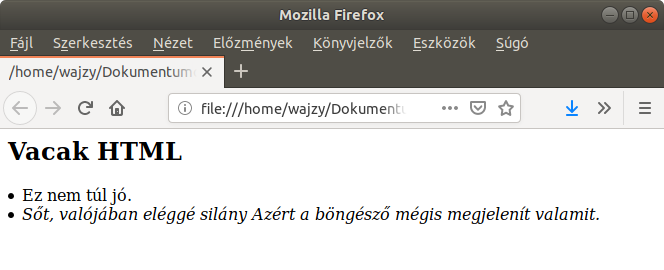
\includegraphics[width=\textwidth]{hibas_firefox.png} \\
        Mozilla Firefox 69.0
      \end{center}
    \column{0.3\textwidth}
      \begin{center}
        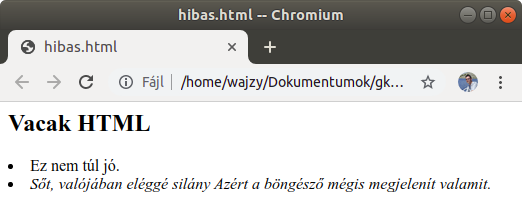
\includegraphics[width=\textwidth]{hibas_chromium.png} \\
        Chromium 76.0.3809.100
      \end{center}
    \column{0.3\textwidth}
      \begin{center}
        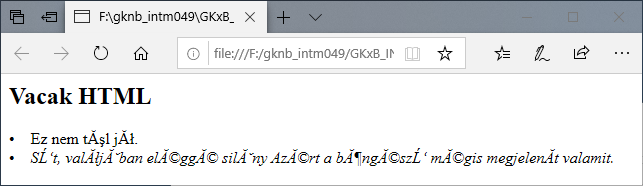
\includegraphics[width=\textwidth]{hibas_edge.png} \\
        Microsoft Edge 44.17763.1.0
      \end{center}
  \end{columns}
\end{frame}

\subsection{Az első HTML oldal elkészítése}

%13
\begin{frame}
  Válasszunk egy szövegszerkesztőt (pl. 
    \hiv{\href{https://www.geany.org/}{Geany}}, 
    \hiv{\href{https://code.visualstudio.com/}{VS Code}}, 
    \hiv{\href{https://notepad-plus-plus.org/}{NotePad++}}, \dots), 
    gépeljük be és mentsük ki az alábbi fájlt \texttt{elso.txt} néven, UTF-8 kódolással!
    \footnotesize
    \begin{exampleblock}{\textattachfile{elso.html}{elso.html}}
      \lstinputlisting[style=HTML]{elso.html}
    \end{exampleblock}
\end{frame}

%14
\begin{frame}
  Dokumentum típusának meghatározása
  \begin{description}[m]
    \item[HTML5] \kiemel{Nincs DTD!} \hfill \\
      <!DOCTYPE html>
    \item[4.01, Szigorú] \hfill \\
      <!DOCTYPE HTML PUBLIC "-//W3C//DTD HTML 4.01//EN" "http://www.w3.org/TR/html4/strict.dtd">
    \item[4.01, Átmeneti] \hfill \\
      <!DOCTYPE HTML PUBLIC "-//W3C//DTD HTML 4.01 Transitional//EN" "http://www.w3.org/TR/html4/loose.dtd">
    \item[4.01, Keretek] \hfill \\
      <!DOCTYPE HTML PUBLIC "-//W3C//DTD HTML 4.01 Frameset//EN" "http://www.w3.org/TR/html4/frameset.dtd">
    \end{description}
\end{frame}

%15
\begin{frame}
  Elemek (element)
  \begin{itemize}
    \item Általában nyitó és záró cimkék (tag) között, pl. \texttt{<body>\dots</body>}, \texttt{<p>\dots</p>}
    \item Néha a böngésző kitalálja, hol kellene lennie az elem (pl. \texttt{<p>}, \texttt{<li>}) záró címkéjének, így az elhagyható, de \kiemel{nem javasolt} (XML elemző számára szabálytalanná teszi a fájlt)
    \item Léteznek üres elemek is; itt nincs mit közbezárni címkékkel, pl. \texttt{<meta />}, vízszintes vonal \texttt{<hr~/>} vagy \texttt{<hr>}
    \item Rögzített szabályok szerint egymásba ágyazhatók
    \item Kis- és nagybetűkre érzéketlen, de \kiemel{ajánlott} a kisbetűs írásmód
    \item A szöveg tördelése független a forrásszöveg tördelésétől (pl. az egymás mellé gépelt fehér karaktereket egynek tekinti)
    \item Címkék mindig \kiemel{<} és \kiemel{>} jelek között
    \item Jelentéssel bíró karakterek bevitele \hiv{\href{https://en.wikipedia.org/wiki/List_of_XML_and_HTML_character_entity_references\#Character_entity_references_in_HTML}{entitásokkal}} (pl. \kiemel{<} $\to$ \kiemel{\&lt;} vagy \kiemel{>} $\to$ \kiemel{\&gt;})
  \end{itemize}
\end{frame}

%16
\begin{frame}
  Elemek
  \begin{description}[m]
    \item[\texttt{<html>}] gyökérelem, pontosan egynek kell lennie (dokumentum nyelve attribútummal, ld. )
    \item[\texttt{<head>}] metaadatok
    \begin{description}
      \item[\texttt{<title>}] dokumentum címe (böngészőablak vagy -fül felirata)
      \item[\texttt{<meta>}] általános metaadat
    \end{description}
    \item[\texttt{<body>}] megjelenítendő tartalom
    \begin{description}
      \item[\texttt{<h1>}] ,,Címsor1''
      \item[\texttt{<p>}] Bekezdés (paragraph)
    \end{description}
  \end{description}
\end{frame}

%17
\begin{frame}
  Attribútumok
  \begin{itemize}
    \item Mindig a nyitó címkében (pl. \texttt{<html lang="hu-HU">}, \hiv{\href{http://www.ietf.org/rfc/rfc1766.txt}{RFC1766}} szerint)
    \item Kulcs-érték párok, = jellel elválasztva
    \item \kiemel{Ajánlott} a kulcsot kisbetűvel írni
    \item Az értéket \kiemel{ajánlott} idézni, lehetőleg ''-vel (de az ' is megfelel; szóközt tartalmazó értéknél pedig kötelező)
    \item Egy címkében lehet több attribútum is
    \item Vagy egy sem (minimalizált szintaxis); itt az attribútum léte hordoz információt (pl. \texttt{<p hidden>}). XML feldolgozók megkövetelik az értéket, pl. \texttt{<p~hidden="hidden">}
  \end{itemize}
\end{frame}

\subsection{Címsorok}

%18
\begin{frame}
  \begin{itemize}
    \item \texttt{<h1>}, \texttt{<h2>}, \dots, \texttt{<h6>}: legmagasabbtól legalacsonyabb szintig
    \item Általában nagyobb betűméretek és a címsor elé és/vagy mögé tett térközök jellemzik
    \item Keresőmotorok is használhatják a dokumentum struktúrájának feltérképezésére
    \item Tematikus részek elválasztására gyakran elválasztó vonalat (\texttt{<hr />}) használnak
  \end{itemize}
\end{frame}

%19
\begin{frame}
  \begin{columns}[c]
    \column{0.5\textwidth}
      Készítsen weboldalt, ami egymás alá írja a \emph{Címsor1}, \emph{Címsor2}, \dots, \emph{Címsor6} szövegeket, a nekik megfelelő HTML elemekkel, a 3. és a 4. szövegsor között pedig húz egy vízszintes vonalat!
    \column{0.5\textwidth}
      \begin{exampleblock}{\textattachfile{cimsorok.html}{cimsorok.html}}
        \begin{center}
          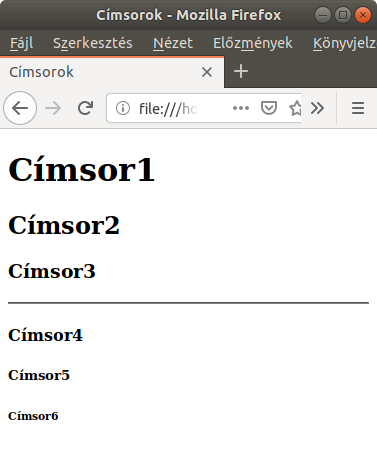
\includegraphics[scale=.25]{cimsorok.png}
        \end{center}
      \end{exampleblock}
  \end{columns}
\end{frame}

\subsection{Bekezdések}

%20
\begin{frame}
  \begin{itemize}
    \item Bekezdések \texttt{<p>} elemmel jelölhetők
    \item \texttt{title} attribútum felugró szövegdoboz, ,,tooltip'' szöveg megadására
    \item Alapértelmezetten térközt hagy a böngésző a bekezdések között
    \item Sortörés új bekezdés (és térköz) nélkül: \texttt{<br />}
    \item Előformázott szöveg (pl. karakteres módú program kimenete), egyenszélességű (monospace) karakterekkel, forrás fehér karaktereinek megőrzésével: \texttt{<pre>}
  \end{itemize}
  \vfill
  ,,Tradicionális'' \hiv{\href{https://developer.mozilla.org/en-US/docs/Web/HTML/Block-level_elements}{tördelési módok}}
  \begin{description}[m]
    \item[Blokkszintű] (block) \hfill \\ Új sorban kezdődik, és a teljes elérhető szélességet elhasználja, pl. \texttt{<p>}, \texttt{<pre>}, \texttt{<h1>}-\texttt{<h6>}, \texttt{<hr />}
    \item[Soron belüli] (inline) \hfill \\ Aktuális sorban kezdődik, csak olyan széles helyet foglal, ahol éppen elfér, pl. \texttt{<br />}
  \end{description}
\end{frame}

%21
\begin{frame}
  \begin{columns}[c]
    \column{0.75\textwidth}
      Formázza meg a \textattachfile{attila.txt}{verset} a mellékelt ábra szerint, azaz
      \begin{itemize}
        \item a költő neve legyen első szintű címsor, 
        \item a mű címe második szintű,
        \item a szakaszok (arab számokkal jelölve) harmadik szintűek.
        \item A bekezdéseket és a bekezdésen belüli sortöreseket állítsa be!
        \item A bekezdések fölé mozgatva az egeret lássuk a bekezdés sorszámát, pl. 1/1, 1/2, \dots, 2/3
      \end{itemize}
    \column{0.25\textwidth}
      \begin{center}
        \begin{exampleblock}{\textattachfile{attila.html}{attila.html}}
          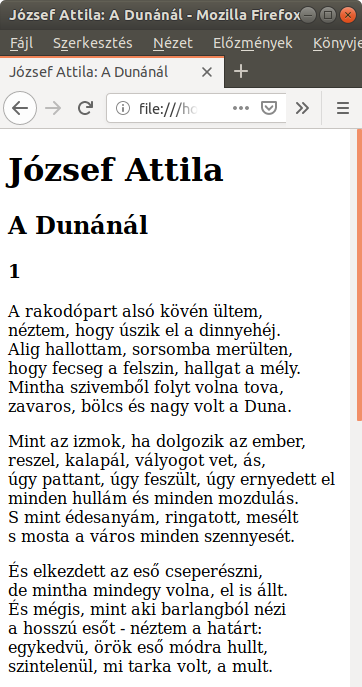
\includegraphics[scale=.2]{attila.png}
        \end{exampleblock}
      \end{center}
  \end{columns}
\end{frame}

% TODO: <pre> elem használata, Fahrenheit-Celsius

\end{document}
